\documentclass[a4paper, twoside]{report}

%% Language and font encodings
\usepackage[english]{babel}
\usepackage[utf8]{inputenc}
\usepackage[T1]{fontenc}

\usepackage[
    backend=biber, 
    eprint=false,
    url=false, 
    sorting=none,
    style=numeric
]{biblatex}
\addbibresource{./bibs/introduction.bib}
\addbibresource{./bibs/background.bib}
\addbibresource{./bibs/evaluation.bib}


%% Sets page size and margins
\usepackage[a4paper,top=3cm,bottom=2cm,left=3cm,right=3cm,marginparwidth=1.75cm]{geometry}

%% Useful packages
\usepackage{amsmath}
\usepackage{amssymb}
\usepackage{graphicx}
\usepackage[colorlinks=true, allcolors=blue]{hyperref}

\usepackage{parskip}
\usepackage{ragged2e}
\usepackage[ruled]{algorithm2e}
\usepackage{array}
\usepackage{booktabs}
\usepackage{longtable}
\usepackage{enumitem}
\usepackage{csquotes}

% Used for checkmarks.
\usepackage{pifont}% http://ctan.org/pkg/pifont
\newcommand{\cmark}{\ding{51}}%
\newcommand{\xmark}{\ding{55}}%

% Used for bullets in tables.
\newcommand{\tabitem}{~~\llap{\textbullet}~~}

\title{Generative Models for Producing Synthetic Retinal Fundus Images \\ \vspace{0.3cm} \Large Interim Report}
\author{Joon-Ho Son}

\begin{document}
\begin{titlepage}

\newcommand{\HRule}{\rule{\linewidth}{0.5mm}} % Defines a new command for the horizontal lines, change thickness here

%----------------------------------------------------------------------------------------
%	LOGO SECTION
%----------------------------------------------------------------------------------------


\includegraphics[width=8cm]{title/logo.eps}\\[1cm] % Include a department/university logo - this will require the graphicx package
 
%----------------------------------------------------------------------------------------

\center % Center everything on the page

%----------------------------------------------------------------------------------------
%	HEADING SECTIONS
%----------------------------------------------------------------------------------------

\textsc{\LARGE MEng Individual Project}\\[1.5cm] % Name of your university/college
\textsc{\Large Imperial College London}\\[0.5cm] % Major heading such as course name
\textsc{\large Department of Computing}\\[0.5cm] % Minor heading such as course title

%----------------------------------------------------------------------------------------
%	TITLE SECTION
%----------------------------------------------------------------------------------------
\makeatletter
\HRule \\[0.4cm]
{ \huge \bfseries \@title}\\[0.4cm] % Title of your document
\HRule \\[1.5cm]
 
%----------------------------------------------------------------------------------------
%	AUTHOR SECTION
%----------------------------------------------------------------------------------------

\begin{minipage}{0.4\textwidth}
\begin{flushleft} \large
\emph{Author:}\\
\@author % Your name
\end{flushleft}
\end{minipage}
~
\begin{minipage}{0.4\textwidth}
\begin{flushright} \large
\emph{Supervisor:} \\
Dr Benjamin Hou \\[1.2em] % Supervisor's Name
\emph{Second Marker:} \\
Dr Amir Alansary % second marker's name
\end{flushright}
\end{minipage}\\[2cm]
\makeatother

% If you don't want a supervisor, uncomment the two lines below and remove the section above
%\Large \emph{Author:}\\
%John \textsc{Smith}\\[3cm] % Your name

%----------------------------------------------------------------------------------------
%	DATE SECTION
%----------------------------------------------------------------------------------------

{\large \today}\\[2cm] % Date, change the \today to a set date if you want to be precise

\vfill % Fill the rest of the page with whitespace

\end{titlepage}

%% Commented for the interim report

% \begin{abstract}
% Your abstract goes here
% \end{abstract}

% \renewcommand{\abstractname}{Acknowledgements}
% \begin{abstract}
% Thanks mum!
% \end{abstract}

\tableofcontents
% \listoffigures
% \listoftables

\chapter{Introduction}

% The introduction should summarise the subject area, the specific problem you are addressing, including key ideas for their solution, together with a summary of the project's main contributions. When detailing the contributions it is helpful to provide forward references to the section(s) of the report that provide the relevant technical details. The introduction should be aimed at an informed, but otherwise non-expert, reader. A good tip is to assume that all your assessors will read the abstract and introduction, whereas the more detailed technical sections may only be read by your first and second markers - it's therefore really important to get it right.

%% What is the problem
% Background on DR itself.

Diabetic retinopathy (DR) is an eye disease that commonly arises as a complication of diabetes. It is estimated that by the year 2045 693 million people worldwide will be living with diabetes. Of these, nearly all of those with type 1 and two-thirds of those with type 2 will be suffering some degree of retinopathy within 20 years of receiving their diagnosis \cite{Mathure014444}. Despite DR being preventable with early detection and intervention, this is made difficult by the fact that the early stages of DR show no symptoms and may only be identified by screening. However, the scalability of mass screening is severely limited by the availability of medical professionals, causing DR to remain as leading cause of blindness in the UK \cite{Liewe004015}. Currently, diagnosis requires manual inspection of retinal fundus images for the presence of abnormalities. This is a time consuming and error-prone process for ophthalmologists who, even when available, have been shown to be inconsistent \cite{DBLP:journals/corr/abs-1710-01711}. For this reason, automated and semi-automated techniques for DR diagnosis have been a popular topic of research, going back as far as .... As more sophisticated and powerful methods are developed, we come ever closer accessible screening for \emph{all} susceptible individuals.

The progression of DR is characterised by the formation of lesions on a patient's retina, the type and quantity of which indicate the severity of the disease. The ability to identify the precise locations of these lesions from the healthy parts of a retina ensures that the most appropriate and interpretable diagnosis possible can be given, as well as having uses in aiding surgical procedures. The task of labelling each pixel of an image to a class label is termed ``semantic segmentation''.

Developments in deep learning over the past decade have sparked a frenzy of breakthroughs in the field of medical imaging. Deep neural networks provide state-of-the-art models across a variety of domains, and continue to show even greater potential. This innovation is fuelled by greater quantities of data, allowing models to generalise to unseen examples. Indeed, in 2017 The Economist coined the phrase ``data is the new oil'', which has become a popular refrain to describe the value of having an abundance of data. This insatiable hunger for data is one of the primary obstacles in the lesion segmentation task, as large-scale, pixel-wise annotated datasets are scarce.

% The need for novel techniques.

An easy way to improve data diversity is by applying data augmentation techniques such as reflections, crops, rotations, and colour perturbations. However, these methods produce images that are highly correlated, and ultimately have low diversity. A more advanced method of image simulation has been to hand-craft complex mathematical models representing the human anatomy, from which images can be sampled. More recently, with the rise of data-driven techniques we have seen a paradigm shift away from this top-down approach to a bottom-up approach of learning the data distribution \emph{directly} from the data itself. This has been made possible by the introduction of Generative Adversarial Networks (GANs). The aim of this project is to leverage these generative models to produce realistic synthetic training data in large volumes.

Achieving large-scale data generation with arbitrary labels would yield significant improvements in the ability of neural networks to both semantically segment retinal fundus images, as well as assign image-level grades. Ultimately \emph{surpass} human ability. This project represents a step towards the goal of fully-automated retinal screening for the detection of diabetic retinopathy by presenting methods to combat the scarcity of data.
\chapter{Background}

% The background section of the report should set the project into context by relating it to existing published work which you read at the start of the project when your approach and methods were being considered. There are usually many ways of solving a given problem, and you shouldn't just pick one at random. Describe and evaluate as many alternative approaches as possible. The published work may be in the form of research papers found in the academic literature, articles, text books, technical manuals, or even existing software or hardware of which you have had hands-on experience. Your must acknowledge the sources of your inspiration. You are expected to have seen and thought about other people's ideas; your contribution will be putting them into practice in some other context. However, avoid plagiarism: if you take another person's work as your own and do not cite your sources of information/inspiration you are being dishonest. When referring to other pieces of work, cite the sources where they are referred to or used, rather than just listing them at the end. Accidental plagiarism or not knowing how to cite and reference is not a valid reason for plagiarism. Make sure you read and digest the Department's plagiarism document .

% In writing the Background chapter you must demonstrate your ability to analyse, synthesise and apply critical judgement. Analysis is shown by explaining how the proposed solution operates in your own words as well as its benefits and consequences. Synthesis is shown through the organisation of your Related Work section and through identifying and generalising common aspects across different solutions. Critical judgement is shown by discussing the limitations of the solutions proposed both in terms of their disadvantages and limits of applicability.

In this chapter, we provide the necessary preliminaries and research context to understand the problem space and proposed solution.

\section{Diabetic Retinopathy} \label{background:classifyingdr}

Diabetic retinopathy is damage to the blood vessels of the retina caused by high blood sugar levels. The level of damage, and hence the stage of DR, can be determined by identifying and categorising different types of lesions on the patient's retina. A description of a subset of these lesions is given as follows \cite{taylor2012handbook}:

\begin{description}
    \item[Microaneurysms (MA)] \hfill \\ Small red round dots caused by weakness in the vessel's walls.
    \item[Haemorrhages (HE)] \hfill \\ Larger spots on the retina.
    \item[Hard exudates (EX)] \hfill \\ Bright yellow spots caused by the leakage of plasma.
    \item[Soft exudates (SE)] \hfill \\ White spots caused by swelling of nerve fibre.
\end{description}

We use color images, not MRI or OCTs or CT scans. Readily available, not as much specialised equipment, telehealth Examples of each type of lesion are shown in \autoref{fig:lesions}.

\begin{figure}
    \centering
    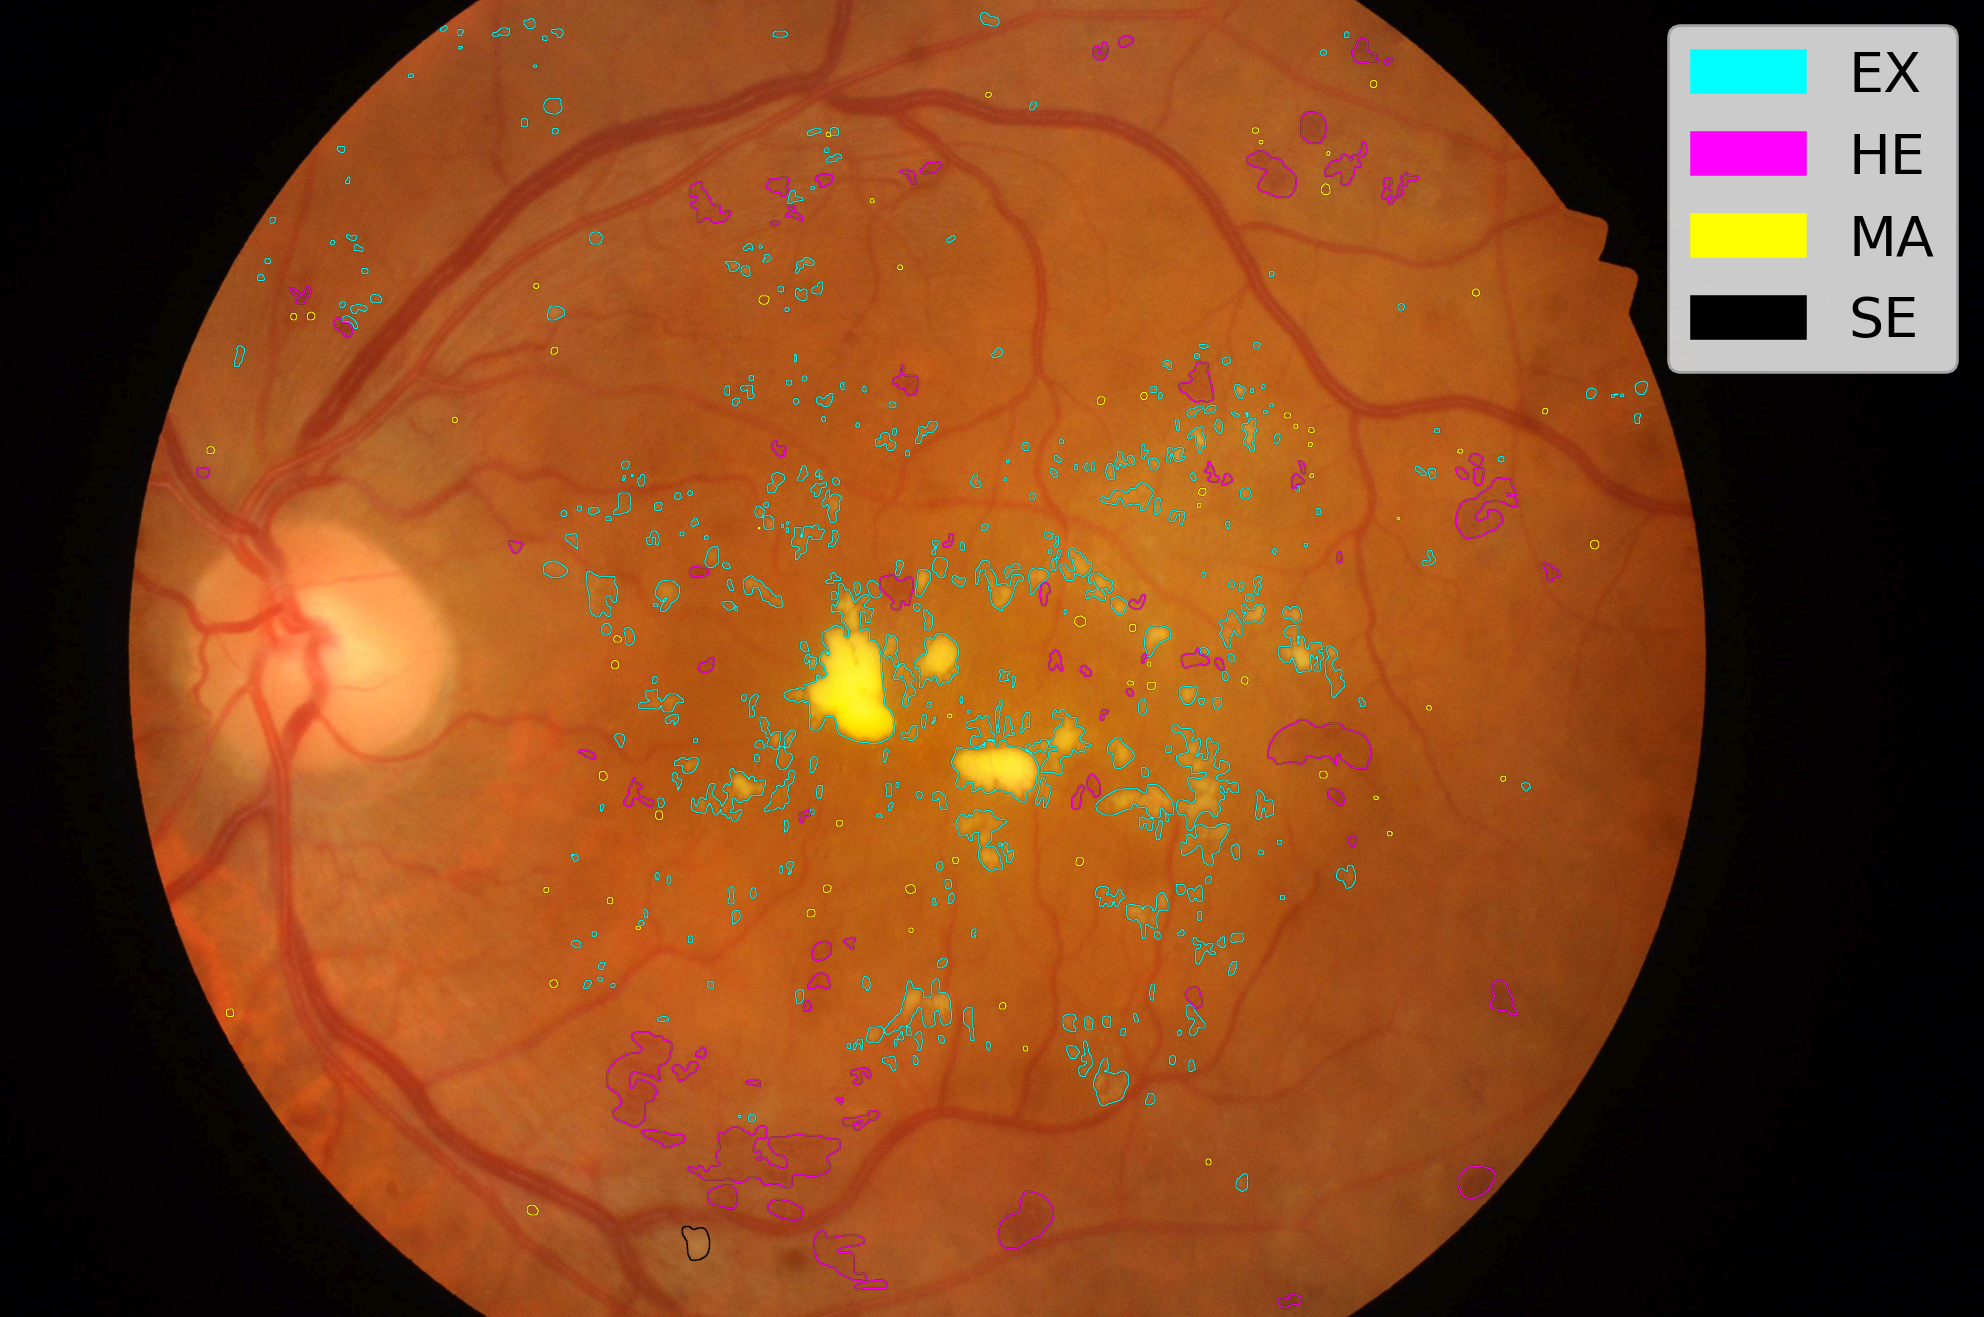
\includegraphics{background/figs/example_output.png}
    \caption{A retinal fundus image annotated with four types of lesions: hard exudates (EX), haemorrhages (HE), microaneurysms (MA), and soft exudates (SE).}
    \label{fig:lesions}
\end{figure}

Clinically, the severity of DR is graded according to an international standard consisting of five stages \cite{ophthalmoscopy2002international}. \autoref{tab:dr_stages} provides a brief summary of the five stages.

\begin{table}
    \centering
    \begin{tabular}{ll}
        \toprule
        Severity & Characteristics \\
        \midrule
        No apparent retinopathy & No abnormalities \\
        Mild NPDR & Microaneurysms only \\
        Moderate NPDR & More than just microaneurysms but less than severe NPDR \\
        Severe NPDR & Any of the following and no signs of PDR: \\ 
        & \tabitem > 20 intraretinal haemorrhages in all 4 quadrants \\
        & \tabitem Venous beading in $\geq$ 2 quadrants\\
        & \tabitem Intraretinal microvascular abnormalities in $\geq$ 1 quadrant \\
        PDR & One or both of: \\
        & \tabitem Neovascularisation \\
        & \tabitem Vitreous/preretinal haemorrhage \\
        \bottomrule
    \end{tabular}
    \caption{The International Clinical Diabetic Retinopathy Disease Scale. \\ NPDR = non-proliferative diabetic retinopathy; PDR = proliferative diabetic retinopathy.}
    \label{tab:dr_stages}
\end{table}

\section{Generative Adversarial Networks}

A Generative Adversarial Network (GAN) is a machine learning framework introduced by Ian Goodfellow in 2014 \cite{NIPS2014_5ca3e9b1} consisting of two neural networks in adversarial competition. The generative model $G$ creates candidate images that look as ``real'' as possible, while the discriminative model $D$ attempts to distinguish between real and synthetic images. Training continues until the discriminator can not longer tell which inputs are fabricated by $G$ and which are real. In this sense, $G$ and $D$ are trained \emph{adversarially}. From this, we can derive the adversarial loss function by taking the cross-entropy of the real and generated functions.
\begin{align} \label{eq:ganloss}
    \mathcal{L}_{GAN} = \mathbb{E}_x[\log D(x)] + \mathbb{E}_z[\log (1-D(G(z))]
\end{align}
where $D(x)$ is the discriminator's estimate that $x$ is real; $G(z)$ is the generator's output when given random noise $z$; $D(G(z))$ is the discriminator's estimate that a fake instance is real. The discriminator will attempt to maximise this loss, whilst the generator will attempt to minimise it. In practice, this happens in alternating phases, keeping the generator fixed when updating the discriminator and vice versa.

The original GAN design is far from perfect, however. In their original paper, \citeauthor{NIPS2014_5ca3e9b1} describe an issue with the original loss formulation where $G$ fails to gain any traction in the early stages of training, and therefore never even begins to converge. This is due to $D$ being able to easily reject to the output of $G$, which causes the gradients to be extremely small. The proposed solution is to, instead of minimising $\log(1-D(G(z))$, \emph{maximise} $\log D(G(z))$.

In no small part to the problems described above, there has been an explosion of GAN variants since their initial introduction. In the following sections, we examine a select few.

\subsection{Conditional GAN}

One of the earliest extensions to the original design, a Conditional GAN (cGAN) extends the vanilla GAN by conditioning on additional information $y$ \cite{mirza2014conditional} This allows us to direct the generation process. Consequently, the loss function previously defined in \autoref{eq:ganloss} now becomes
\begin{align}
    \mathcal{L}_{cGAN} = \mathbb{E}_x[\log D(x|y)] + \mathbb{E}_z[\log (1-D(G(z|y))]
\end{align}

\subsection{ProgressiveGAN}

% Conditional GANs

%% Problems
% Mode collapse.

\section{Image-to-Image Translation}
%  Simulated and Unsupervised Images through Adversarial Training. (2016) Used by Costa
% Image-to-Image Translation with Conditional Adversarial Networks (2016) Used by Costa

\section{Retinal Image Synthesis}

% Automatic Generation of Synthetic Retinal Fundus Images (Fiorini 2014)
% Towards Adversarial Retinal Image Synthesis (Costa 2017)
% Adversarial Synthesis of Retinal Images from Vessel Trees
% End-to-End Adversarial Retinal Image Synthesis (Costa 2017)
% Unsupervised histopathology image synthesis (2017)
% Synthesizing retinal and neuronal images with generative adversarial nets (Tub-GAN) (2018)
% Retinal image synthesis from multiple-landmarks input with generative adversarial networks (2019)
% DR GAN (2020)

Early work surrounding the generation of synthetic retinal fundus images involved patch-based techniques and creating complex mathematical models representing the anatomy of the eye \cite{BONALDI201654, N20103:2014}. Different algorithms had to be proposed for different components of the eye, and computationally expensive operations were used. Heavy use of domain knowledge.

More recently, purely data-driven approaches have been shown to be highly effective. In 2017, \citeauthor{DBLP:journals/corr/CostaGMANMC17} published their foundational work utilising GANs for retinal image synthesis \cite{DBLP:journals/corr/CostaGMANMC17}. The proposed generator network operated by performing image-to-image translation from a vessel network to a retina image. They borrow from CITE, CITE, mentioned above by implementing an adversarial loss function that not only . 

In the absence of a large dataset containing manual annotations, vessel segmentation masks were inferred from the output of a segmentation model. Hence, from a single vessel network, an unbounded number of complete retinal fundus images sharing the same vascular structure could be obtained. However, this approach still suffered some major drawbacks. The generator relies on a vessel segmentation mask as input. This is unideal since the user will have to either (a) manually obtain their own vessel segmentation, which in and of itself is a lot of work, (b) use a pre-existing vessel segmentation, which there is a limited pool of, or (c) infer a vessel segmentation (as the authors did) which may be unreliable. It's worth noting that a poorly inferred vessel network, as may be produced by a segmentation model, fails to produce a usable fundus image as pointed out by the paper's authors. Moreover, the output images have a resolution of $512 \times 512$ which, while large relative to the images often used in computer vision publications, is small compared to those produced by modern fundus photography.

The same authors continued to refine these techniques in a later work \cite{8055572}. The major extension offered by this paper was removing the dependency on a pre-existing vessel segmentation as input. Instead, an adversarial autoencoder is employed to generate vessels segmentation masks, which can be fed into the previously described image-to-image model, requiring the user to simply supply a sample from a multivariate normal distribution. While this overcomes the first of the issues with the previous work by obviating the need to obtain a segmentation mask, the issue of resolution remains. Furthermore, it is noted that the autoencoder does not always generate anatomically correct vascular structures.

\citeauthor{ZHAO201814} incrementally built upon this work in 2018 by introducing Tub-GAN. It is similar to its predecessor in that the same adversarial loss function is sued. The notable improvements are the fact that manual annotations are used. Different outputs from the same input. 

They both use the same loss-function. Both use basic generator architecture but slightly modified. Tub-GAN uses tanh instead of sigmoid.

A few shortcomings are noted. First, the optic disc is blurred.

While representing an important step towards the generation of synthetic fundus images, these methods do not have any relation to DR i.e. generating pathological instances.

DR-GAN uses more recent developments in machine learning like multi-spatial attention.
\chapter{Project Plan}
\chapter{Evaluation Plan}
 Gaidon et al. [5] show that pre-training a deep
neural network on synthetic data leads to improved performance. 
\section{Datasets}

While image-level graded images are widely available, the lesion segmentation task suffers from a paucity of pixel-wise segmented data.

\subsection{IDRiD}

The Indian Diabetic Retinopathy Image Dataset (IDRiD) \cite{Porwal2018} was initially released in 2018 as part of the ``Diabetic Retinopathy: Segmentation and Grading Challenge'' held at ISBI-2018. It consists of 81 retinal fundus images with signs of DR, each of which are accompanied by binary masks for microaneurysms, soft exudates, hard exudates, and haemorrhages (where present) corresponding to pixel-level annotations. All 81 images also have masks for optic disks. Each image has a resolution of $4288\times 2848$.

\subsection{FGADR}

The Fine-Grained Annotated Diabetic Retinopathy (FGADR) \cite{9257400} dataset is a recent dataset released in 2020 by the authors of DR-GAN alongside their publication.

\section{Metrics}
\chapter{Ethical Issues} \label{sec:ethics}

In this chapter we aim to give a brief overview of the ethical implications of the techniques presented in this project, as well as those surrounding machine learning in healthcare more broadly.
% \chapter{Conclusion}
\appendix

\chapter{Ethics Checklist}
\autoref{tab:ethicschecklist} presents an abridged version of the \emph{Ethics Checklist} provided by the Department of Computing. Issued identified in the checklist are discussed in length in \autoref{sec:ethics}.

\begin{longtable}{p{0.01\textwidth}>{\raggedright}p{0.85\textwidth}r}
\toprule
   \multicolumn{2}{l}{Section 1: Humans} \\
   & Does your project involve human participants? & \cmark \\
\midrule
   \multicolumn{2}{l}{Section 2: Protection of Personal Data} \\
   & Does your project involve personal data collection and/or processing? & \cmark \\
   & Does it involve the collection and/or processing of sensitive personal data? & \cmark \\
   & Does it involve processing of genetic information? & \xmark \\
   & Does it involve tracking or observation of participants? & \xmark \\
   & Does your project involve further processing of previously collected personal data (secondary use)? & \cmark \\
   \multicolumn{2}{l}{Section 3: Animals} \\
   & Does your project involve animals? & \xmark \\
   \multicolumn{2}{l}{Section 4: Developing Countries} \\
   & Does your project involve developing countries? & \cmark \\
   & If your project involves low and/or lower-middle income countries, are any benefit-sharing actions planned? & \xmark \\
   & Could the situation in the country put the individuals taking part in the project at risk? & \xmark \\
\midrule 
   \multicolumn{2}{l}{Section 5: Environmental Protection and Safety} \\
   & Does your project involve the use of elements that may cause harm to the environment, animals or plants? & \xmark \\
   & Does your project involve the use of elements that may cause harm to humans, including project staff? & \xmark \\
\midrule 
   \multicolumn{2}{l}{Section 6: Dual Use} \\
   & Does your project have the potential for military applications? & \xmark \\
   & Does your project have an exclusive civilian application focus? & \cmark \\
   & Will your project use or produce goods or information that will require export licenses in accordance with legislation on dual use items? & \xmark \\
   & Does your project affect current standards in military ethics? & \xmark \\
\midrule 
   \multicolumn{2}{l}{Section 7: Misuse} \\
   & Does your project have the potential for malevolent/criminal/terrorist abuse? & \xmark \\
   & Does your project involve information on/or the use of biological-, chemical-, nuclear/radiological-security sensitive materials and explosives, and means of their delivery? & \xmark \\
   & Does your project involve the development of technologies or the creation of information that could have severe negative impacts on human rights standards, if misapplied? & \xmark \\
   & Does your project have the potential for terrorist or criminal abuse? & \xmark \\
\midrule 
   \multicolumn{2}{l}{Section 8: Legal Issues} \\
   & Will your project use or produce software for which there are copyright licensing implications? & \cmark \\
   & Will your project use or produce goods or information for which there are data protection, or other legal implications? & \cmark \\
\midrule 
   \multicolumn{2}{l}{Section 9: Other Ethics} \\
   & Are there any other ethics issues that should be taken into consideration? & \xmark \\
\bottomrule \\

\caption{Ethics Checklist}
\label{tab:ethicschecklist}
\end{longtable}



\printbibliography

\end{document}